\documentclass[convert]{standalone}

\usepackage{tikz}
\usepackage{graphicx}
\pagestyle{empty}

% INT_AY22_L34-Fig01_Uranium-mass-spec.png

\begin{document}
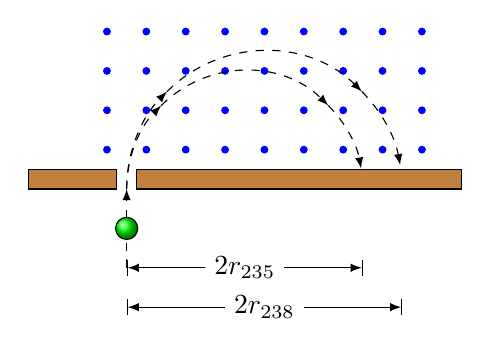
\begin{tikzpicture}[> = latex]

	% Definitions
	
	\def\lattice{0.5}		% Lattice spacing for magnetic field dots
	\def\xmax{9}		% x dimension of bounding box in lattice spacings
	\def\ymax{4}		% y dimension of bounding box in lattice spacings

	% Magnetic field
	
	% Each magnetic field indicator is placed in lattice with \lattice spacing,
	% starting \lattice from bounding box
	
	\foreach \x in {1, 2, ..., \xmax}
	\foreach \y in {1, 2, ..., \ymax}
		\filldraw [blue] (\x * \lattice, \y * \lattice) circle (1.2 pt);
		
	% Mass spectrometer wall
	
	\draw [fill = brown] (-0.5, 0.25) rectangle (0.625, 0);
	\draw [fill = brown] (0.875, 0.25) rectangle (5, 0);
	
	% Uranium ion arcs
	
	\begin{scope}[dashed, ->]
	
		\draw (0.75, -1) -- (0.75, 0);
		\draw (0.75, 0) arc (180 : 135 : {3.5 * \lattice}) coordinate (arc1-1);
		\draw (arc1-1) arc (135 : 45 : {3.5 * \lattice}) coordinate (arc1-2);
		\draw (arc1-2) arc (45 : 10 : {3.5 * \lattice});
		
		\draw (0.75, 0) arc (180 : 135 : {3 * \lattice}) coordinate (arc2-1);
		\draw (arc2-1) arc (135 : 45 : {3 * \lattice}) coordinate (arc2-2);
		\draw (arc2-2) arc (45 : 10 : {3 * \lattice});
	
	\end{scope}
	
	% Entering ion
	
	\draw [ball color = green] (0.75, -0.5) circle (4 pt);
	
	% Distance indicators
	
	\draw [|<->|] (0.75, -1) -- node [fill = white] {$2r_{235}$} ({0.75 + 6 * \lattice}, -1);
	\draw [|<->|] (0.75, -1.5) -- node [fill = white] {$2r_{238}$} ({0.75 + 7 * \lattice}, -1.5);

\end{tikzpicture}
\end{document}